%!TEX root = ../report.tex


\chapter{Design}\label{ch:design}


\section{Design artefacts}\label{sec:design-artefacts}

This part of the document will present the artefacts which have been developed during the design phase.

\begin{figure}[h]
    \centering
    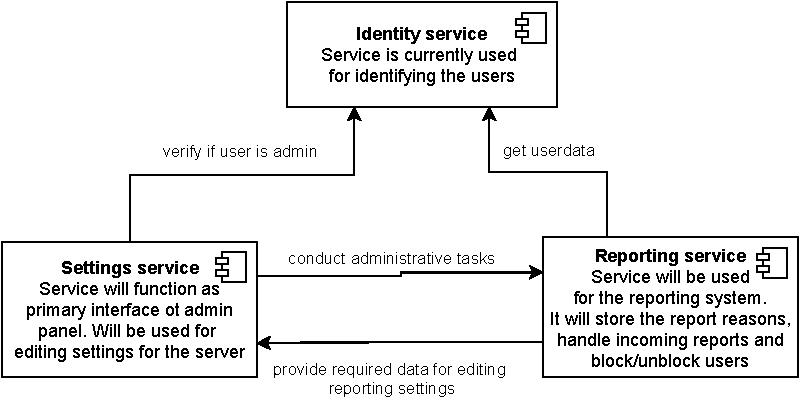
\includegraphics[width=1.0\textwidth]{./graphics/component_interaction}
    \caption{Service interaction concept designed for admin panel}
    \label{fig:componentInteraction}
\end{figure}

The \hyperref[subsubsec:settingsSer]{\textbf{settings service}} will function as the REST interface to the admin panel.
To this point it will interact with the identity service for verifying if the settings are actually being changed by an
administrator user.
It will also work with the \hyperref[subsubsec:reportingSer]{\textbf{reporting service}}: the service in charge of
handling the reporting system, to conduct administrative tasks like changing the reasons people can be reported for.

\begin{figure}[H]
    \centering
    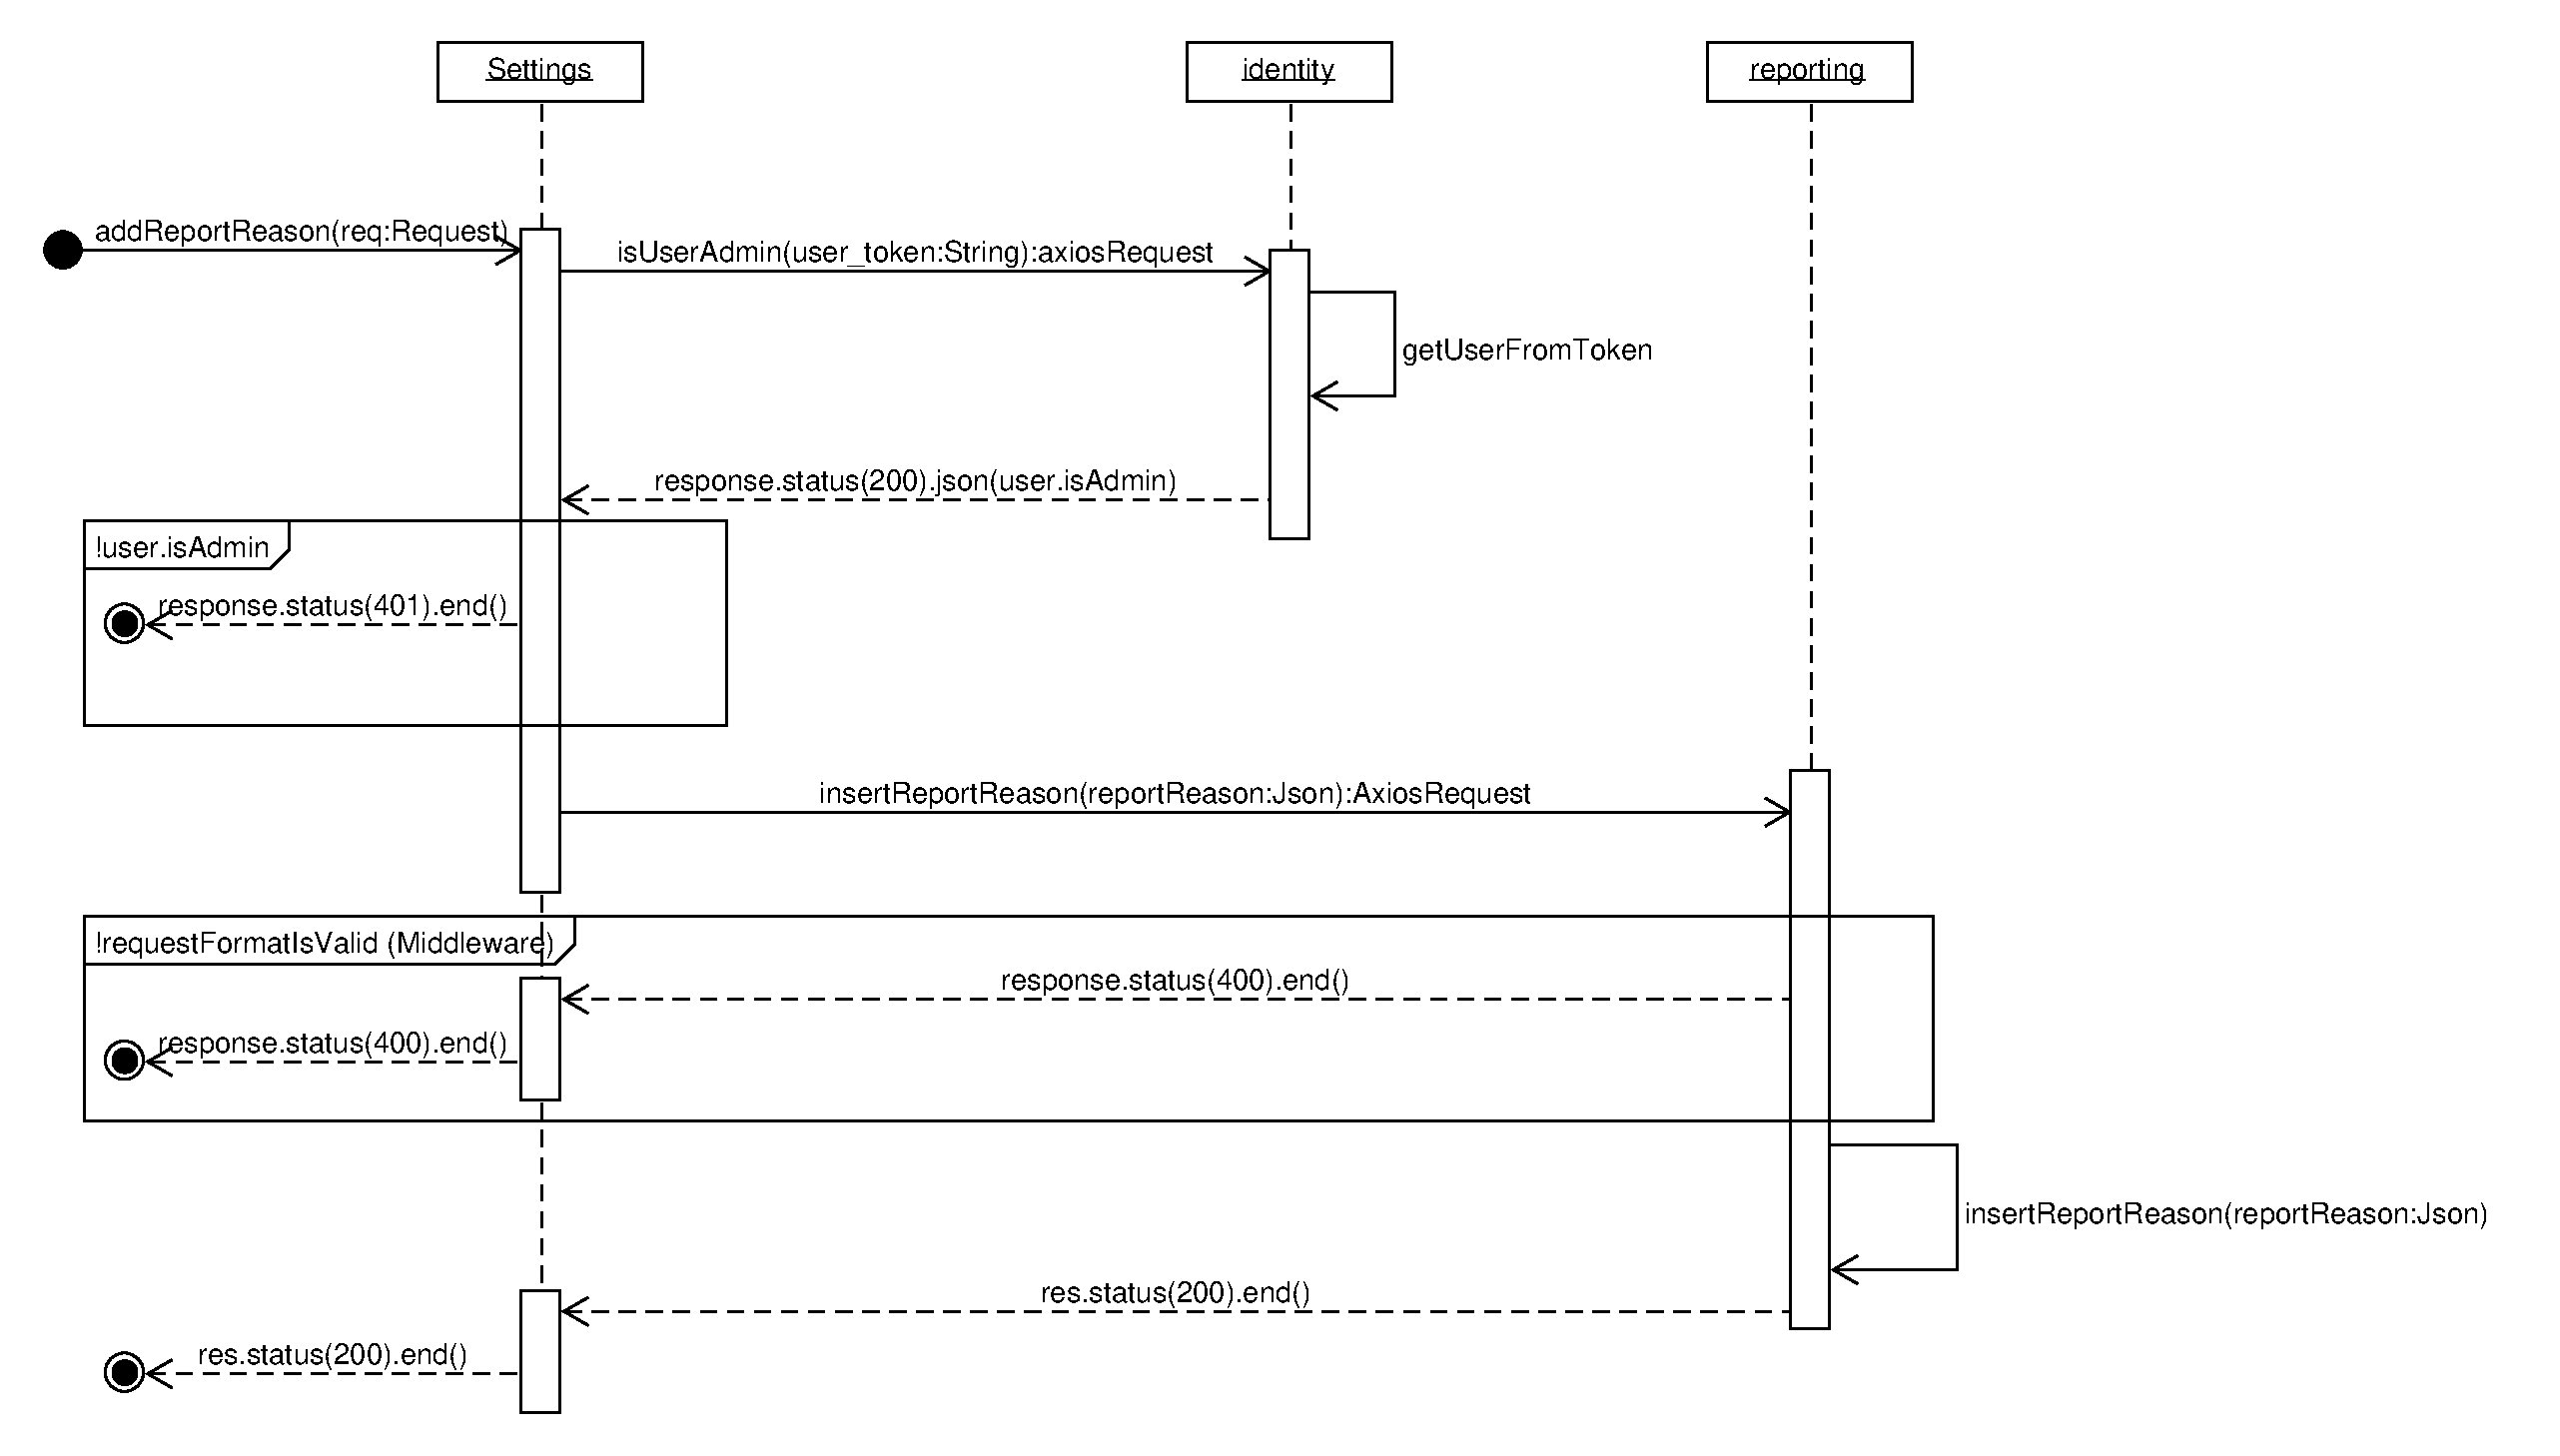
\includegraphics[width=1.0\textwidth]{./graphics/SequenceDiagram_AddReportReason}
    \caption{Service interaction concept designed for admin panel}
    \label{fig:sequenceDiagramAddReportReason}
\end{figure}

Figure~\ref{fig:sequenceDiagramAddReportReason} shows the sequence diagram for conducting the administrative task of
adding a report reason.
This diagram has been created in order to further visualize the responsibility and interaction between the existing
\hyperref[subsubsec:identitySer]{\textbf{identity service}}, and the two other services (settings and reporting).
Further information on this can be derived from~\hyperref[subsubsec:settingsSer]{\textbf{settings service}}.

\begin{figure}[H]
    \centering
    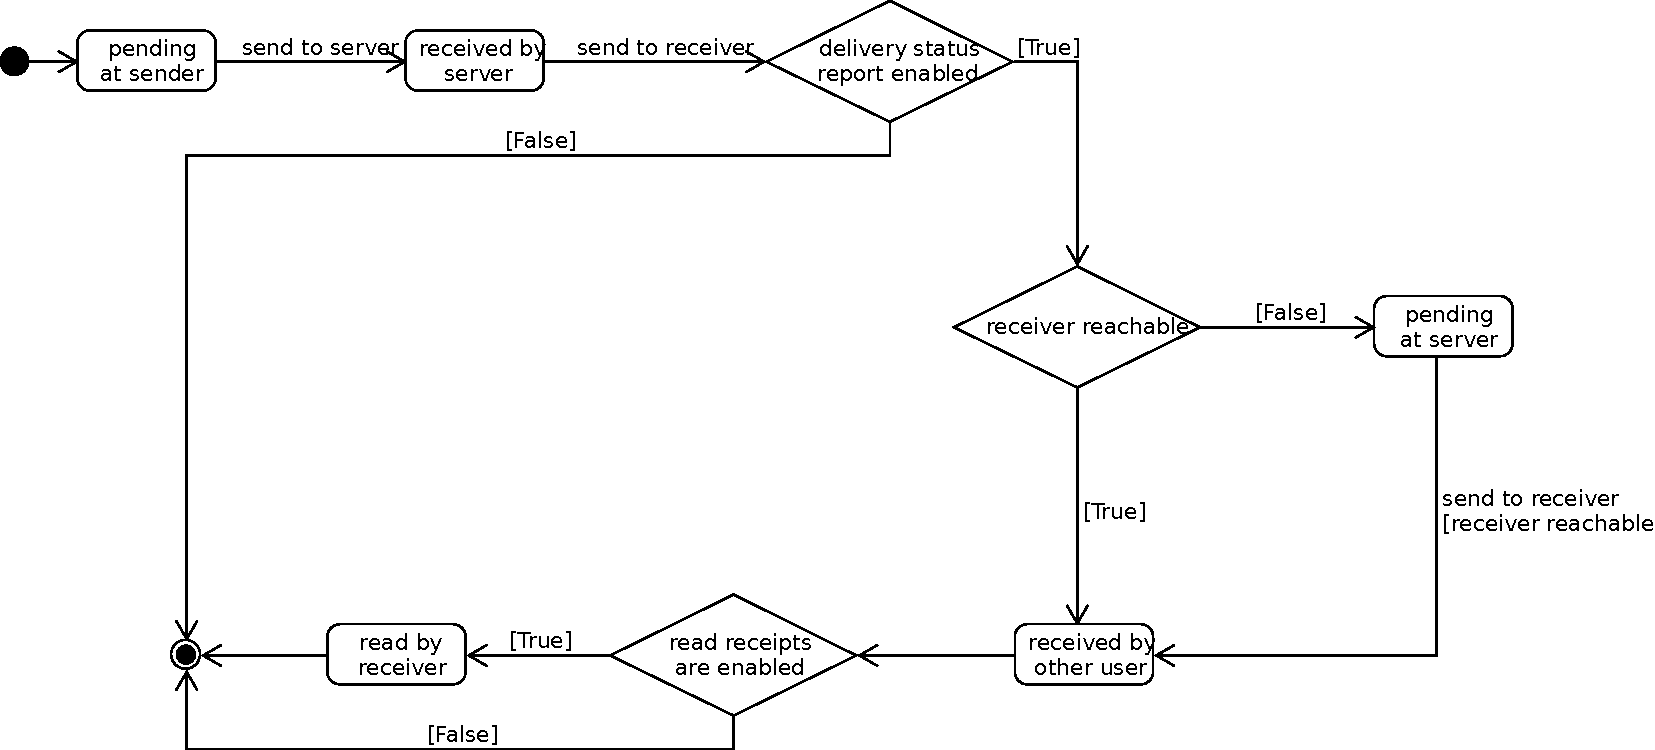
\includegraphics[width=1.0\textwidth]{./graphics/stateMachineMessage}
    \caption{State machine diagram for the message}
    \label{fig:stateMachineMessage}
\end{figure}

Figure~\ref{fig:stateMachineMessage} shows the different states of the message.
First the message will be in the \textit{pending at sender} stage, once the message has been successfully sent to the
server, it will enter the \textit{received by server} stage.
From there on it depends on the settings of the user, whether the delivers status report is enabled or not.
Should this option be disabled, the diagram ends here, otherwise, it will be checked if the receiver is reachable or
not.
If he is not reachable the state will be set to \textit{pending at server} until the message has been received by the
intended user, in which case the state will jump to \textit{received by other user}.
Should the other user be immediately reachable, the state of the message will directly change to the
\textit{received by other user state}.
Next, it again depends on the settings, whether read receipts are enabled or not.
If they are not enabled the diagram ends here, otherwise the message state will be set to \textit{read by receiver}
and the diagram ends here.

\begin{figure}[H]
    \centering
    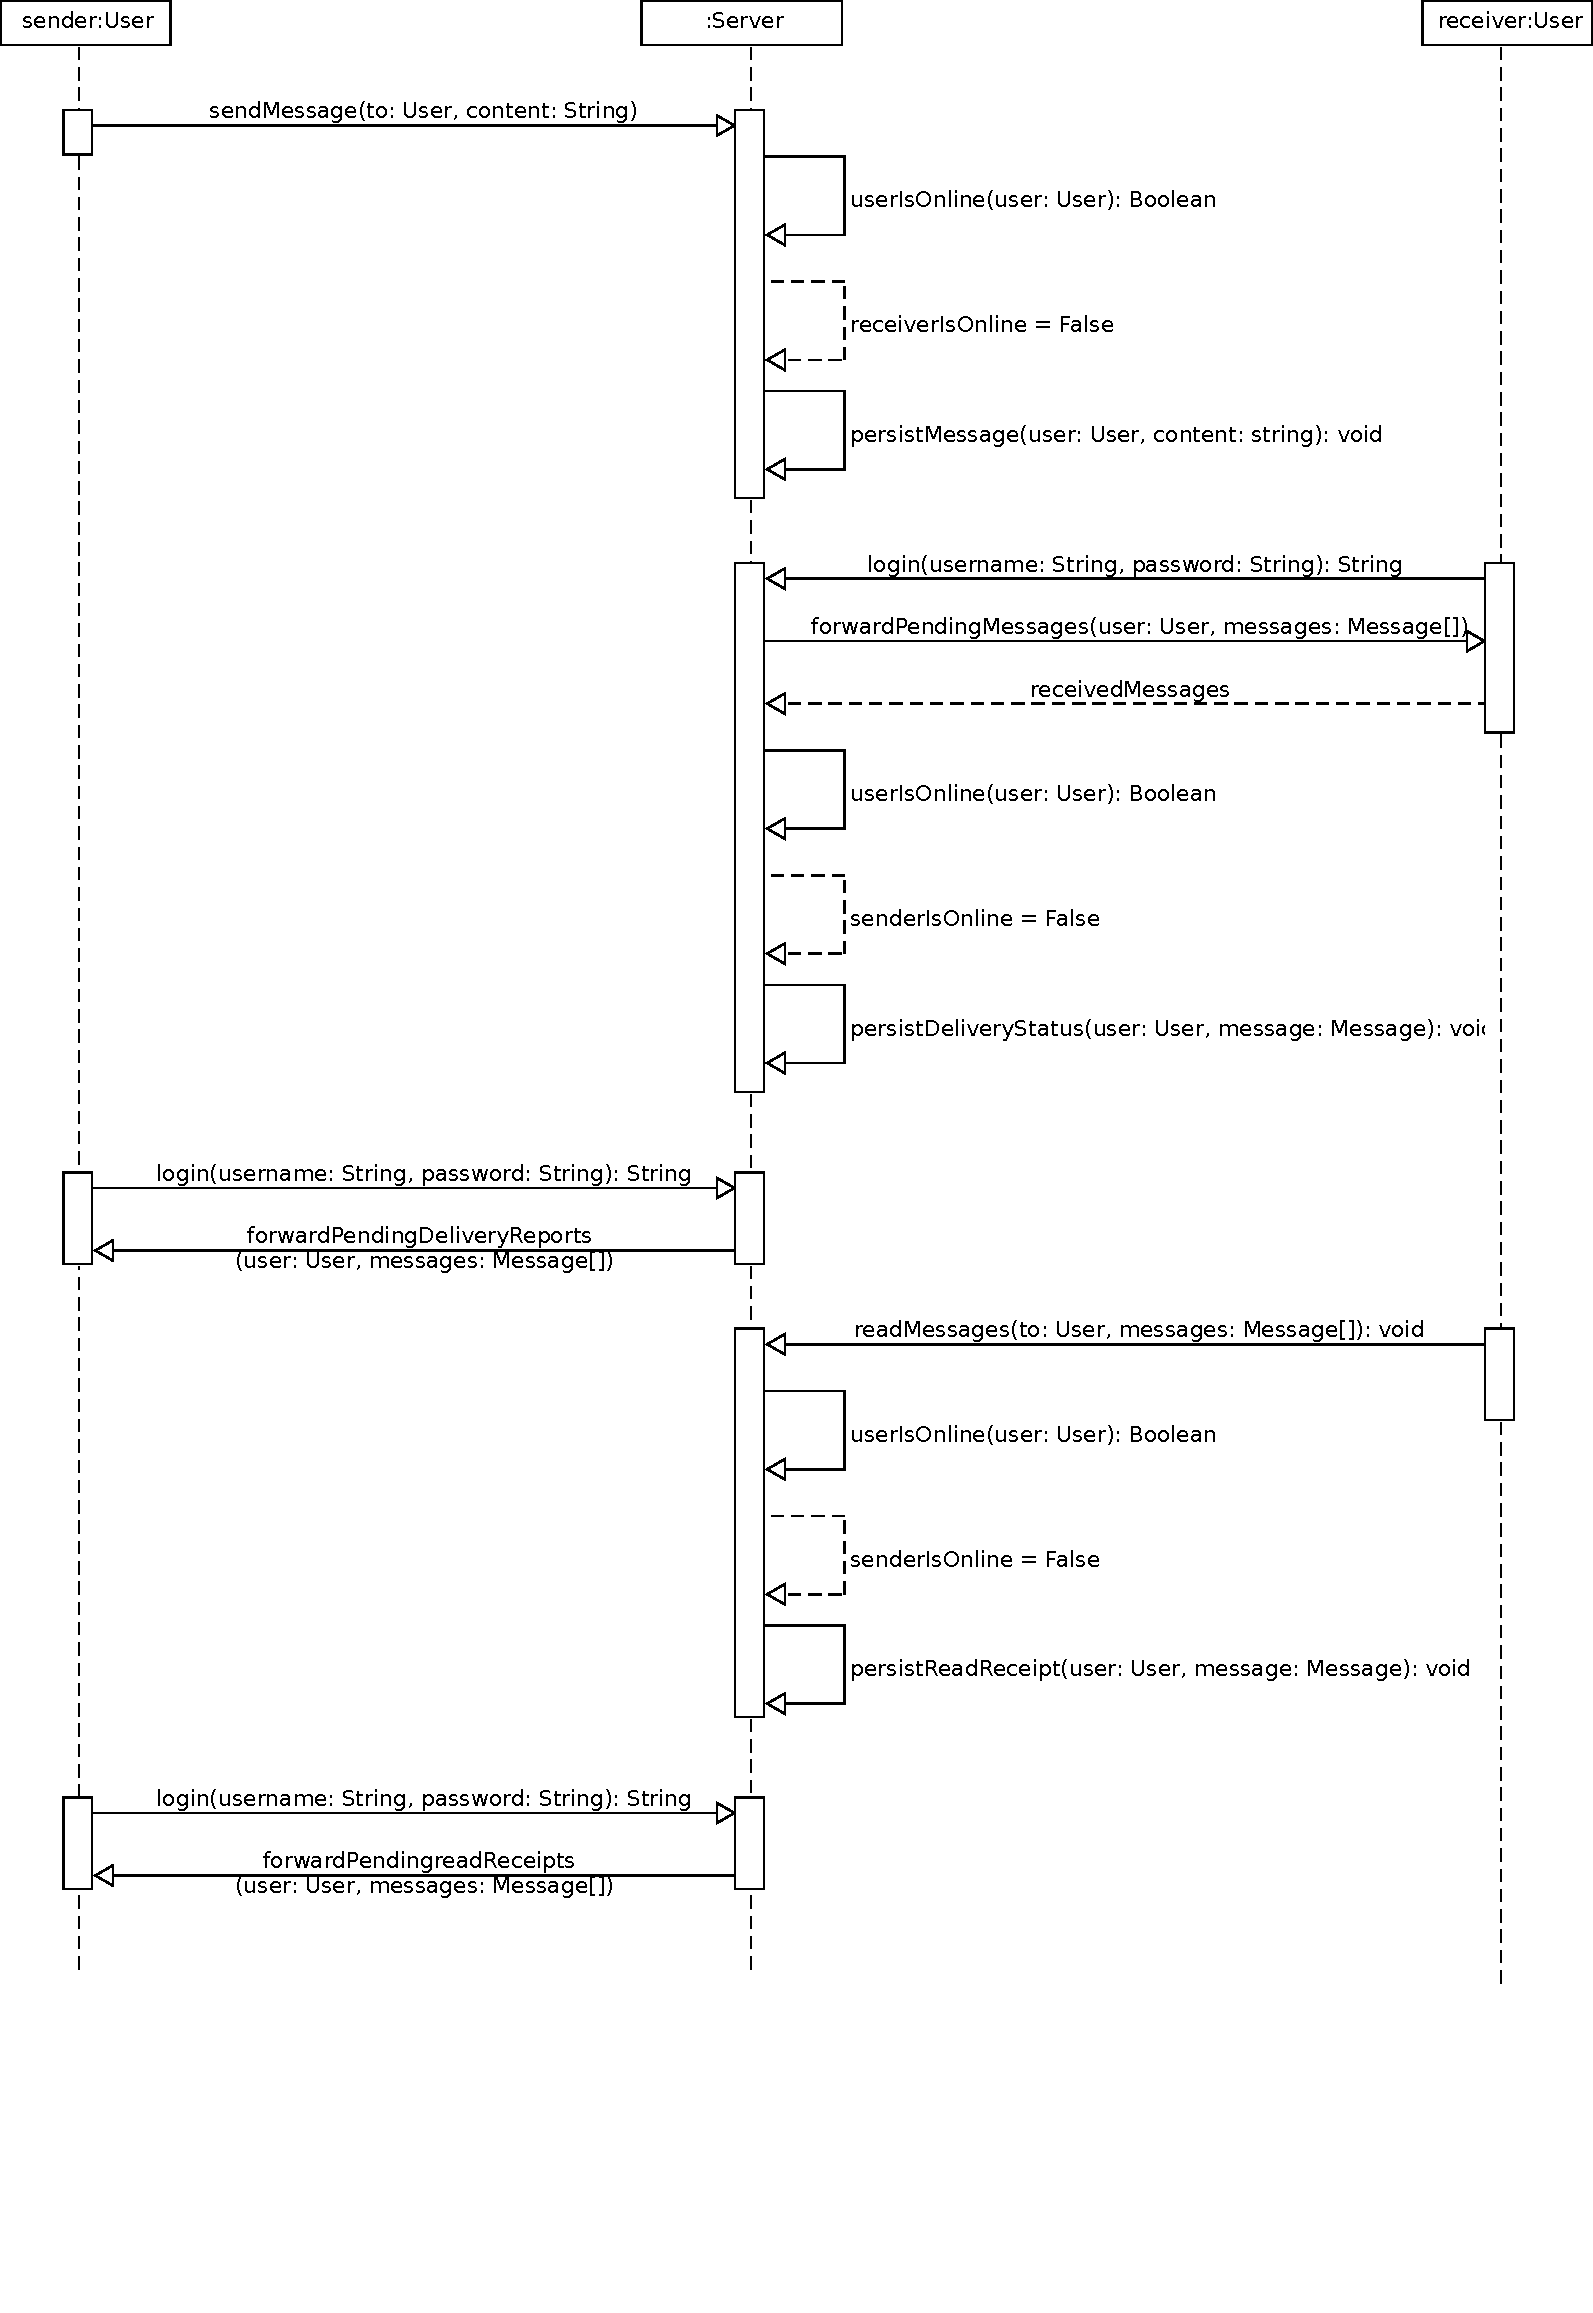
\includegraphics[width=1.0\textwidth]{./graphics/sequenceDiagramMessage}
    \caption{Sequence diagram for sending messages}
    \label{fig:sequenceDiagramMessage}
\end{figure}

Figure~\ref{fig:sequenceDiagramMessage} shows the sequence of sending a message.
This diagram will assume that all the worst cases (receiver is not online for receiving the message and sender is not
there for receiving status updates on the receipt and read receipt status of the message) in order to present how
forwarding of this information will be handled.
The sender sends the message to a certain recipient.
The server then checks if the receiver is online.
In this case he is not (receiverIsOnline = false).
The server will now temporarily store the message (persistMessage) until the recipient has logged in.
As soon as the recipient has logged in the server will forward the pending messages to the receiver.
The receiver client will then let the server know that the message has been received.
The server will now check if the sender is online to forward the delivery update.
In this case the sender is offline (senderIsOnline = false).
The server will now temporarily store the delivery update.
Once the sender has logged in, this will prompt the server to forward the delivery status to the sender.
The recipient at a later point in time will read the message and forward this a read status to the server.
The server will check if the sender is online which he in this case again is not.
Once the sender is logged in the sender will then forward the read receipt status.


\section{Network Design}\label{sec:network-design}

This section covers in detail how the actual software components are set up and how they are linked together.

\subsection{Application System Layers}\label{subsec:application-system-layers}

The following visualization (\ref{fig:figure33}) shows the interaction between the different components in the client
and server application.
It shows in detail how the different concrete parts depend on and communicate with each other.

\begin{figure}[H]
    \centering
    \caption{Trale System Layers and Deployment Diagram}
    \hspace*{-2.9cm}
    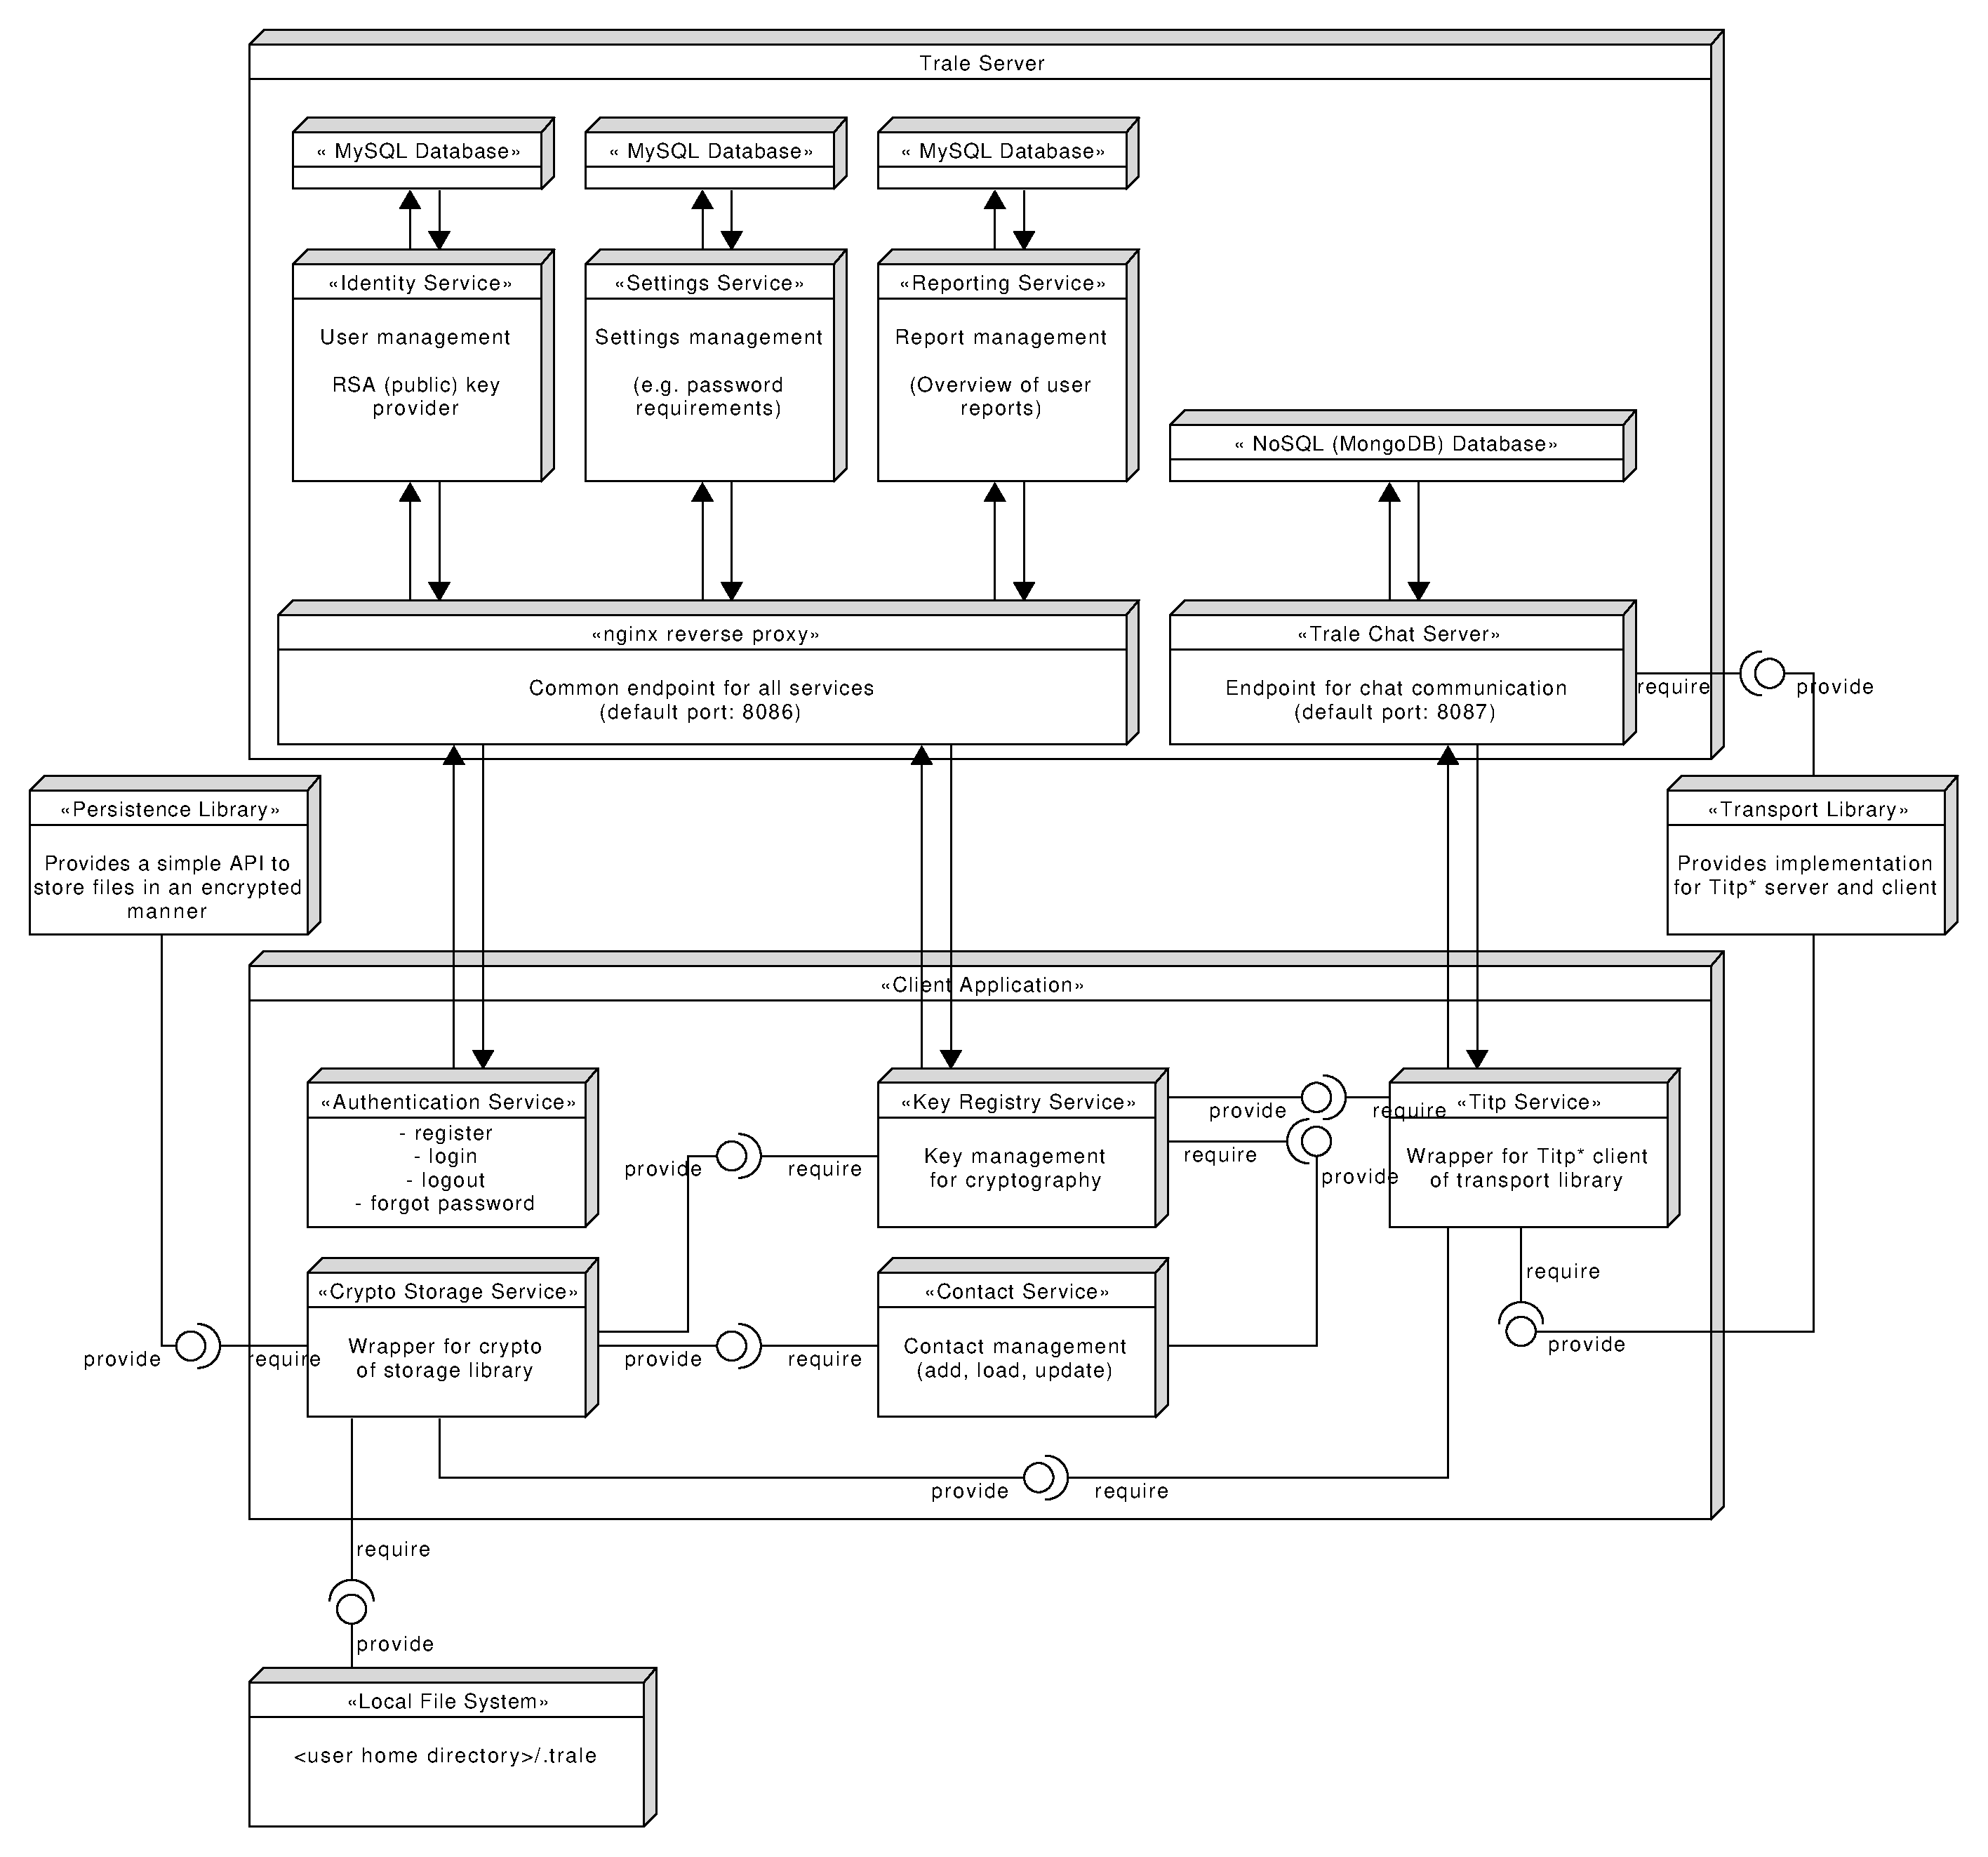
\includegraphics[width=1.3\textwidth]{./graphics/systemLayers}
    \label{fig:figure33}
\end{figure}
\textit{*Titp} stands for \ac{titp}, which will be covered in the section
\hyperref[subsec:transport]{\textbf{transport library}}.

\subsection{Network Architecture}\label{subsec:network-architecture}

The previous diagram (\ref{fig:figure33}) showed how the system is build up in general.
The following diagram shows how participants on many systems may communicate with one-another.

In the example below (\ref{fig:figure32}), Alice and Bob are connected to the same server (A).
They can communicate with each other.
However, they can also communicate with Charly who is located on a different server (B).
The servers are communicating with each other on the users behalf and forward the messages without fully knowing
the conversation partners.
With this approach the sender stays pseudo-anonymous to the receiver and the receiver's server and the opposite way
around.

\begin{figure}[H]
    \centering
    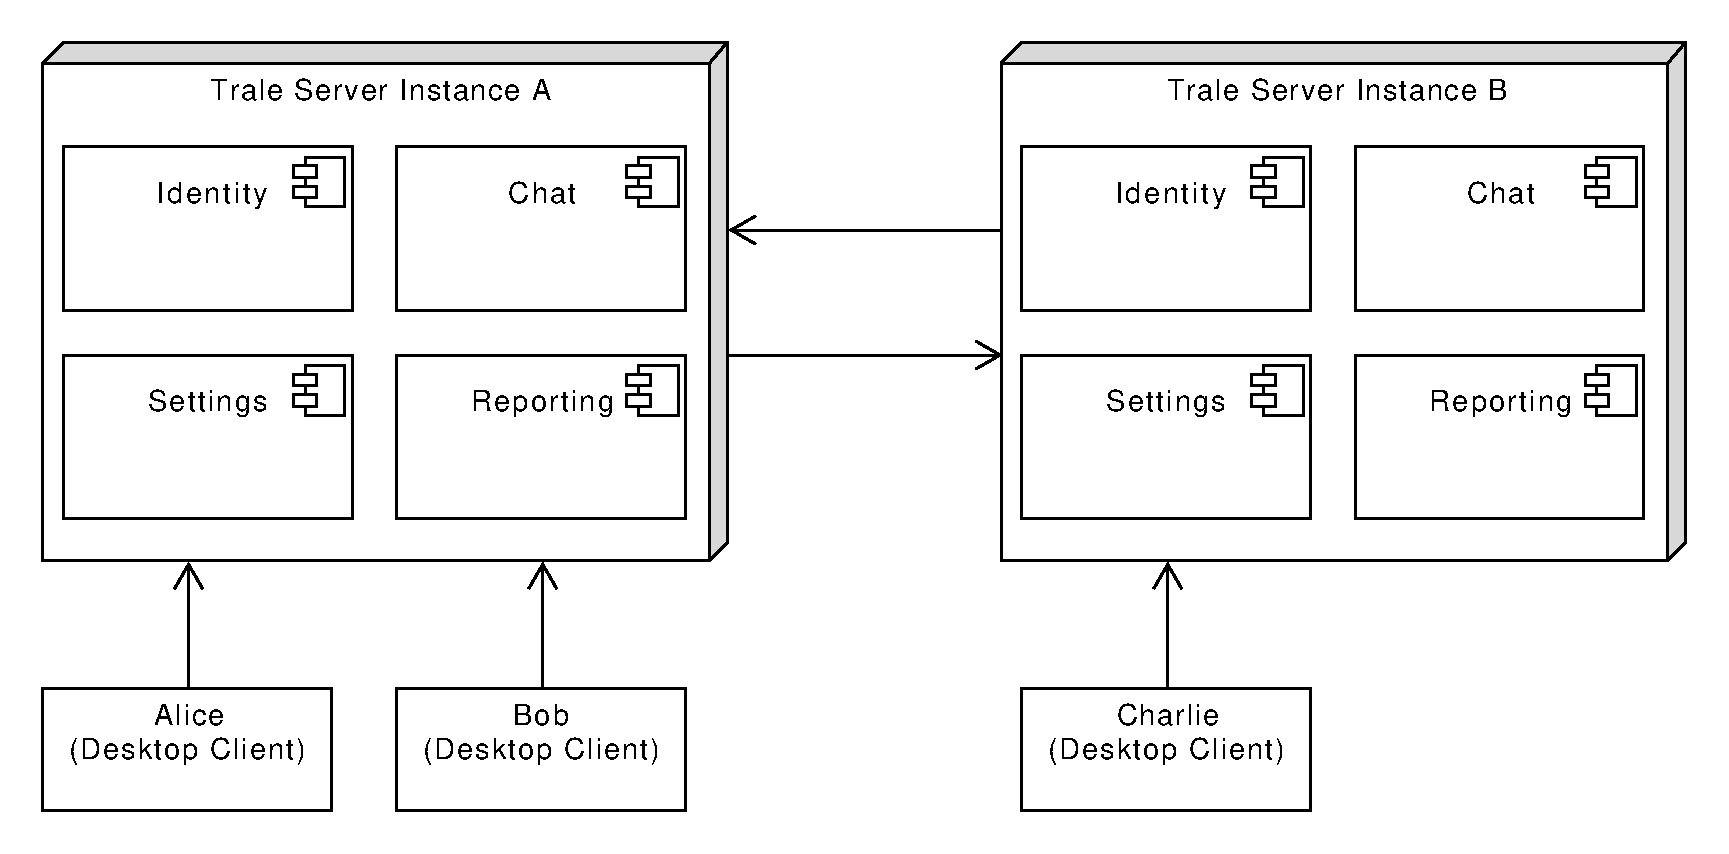
\includegraphics[width=1.0\textwidth]{./graphics/components}
    \caption{Trale Network Architecture}
    \label{fig:figure32}
\end{figure}

\subsection{Port distribution}\label{subsec:port-distribution}

The following table shows all utilized ports of the server side.
External ports are reachable from client applications.
The internal ports are used for inter-service communication.

\begin{table}[H]
    \centering
    \begin{tabular}{|l|l|l|}
        \toprule
        \textbf{Port} & \textbf{Port Type} & \textbf{Service}                               \\
        \midrule
        8086          & External & Default \ac{http} Port (see~\ref{fig:figure33})     \\
        \midrule
        8087          & External & Default \ac{titp} Port (see~\ref{fig:figure33})     \\
        \midrule
        3000          & Internal & Identity Service                               \\
        \midrule
        3001          & Internal & Chat service over \ac{http}                         \\
        \midrule
        3002          & Internal & Chat service over Trale connection \\
        \bottomrule
    \end{tabular}\label{tab:table}
\end{table}

\subsection{Trale Library Design}\label{subsec:trale-library-design}

This section will cover a detailed overview over all self-developed libraries.
The trale library utilizes a combination of synchronous encryption, \ac{aes} and asynchronous encryption \ac{rsa}.

\subsubsection{Transport Library}

\paragraph{User Key Registry}
The user key registry is a functional interface.
It only provides one method to fetch a user's \ac{rsa} public key.
It is used for end-to-end encryption where no shared secret is available (i.e.\ there has not been a key negotiation
yet).
In other cases synchronous encryption is not applicable (e.g.\ sender name in a message), so for secure asymmetric
encryption the public key of the recipient needs to be fetched.

\paragraph{Conversation Key Registry}
The conversation key registry serves multiple purposes in the realm of managing various keys needed for conversation
initialization.
Mainly, it is responsible for loading and updating synchronous conversation keys.
Additionally, it takes care of temporarily storing \ac{ecdh} key pairs during handshake initialization.
This is necessary in case one starts a handshake with another user who is currently not reachable, so the handshake can
be completed later on.

\begin{figure}[H]
    \centering
    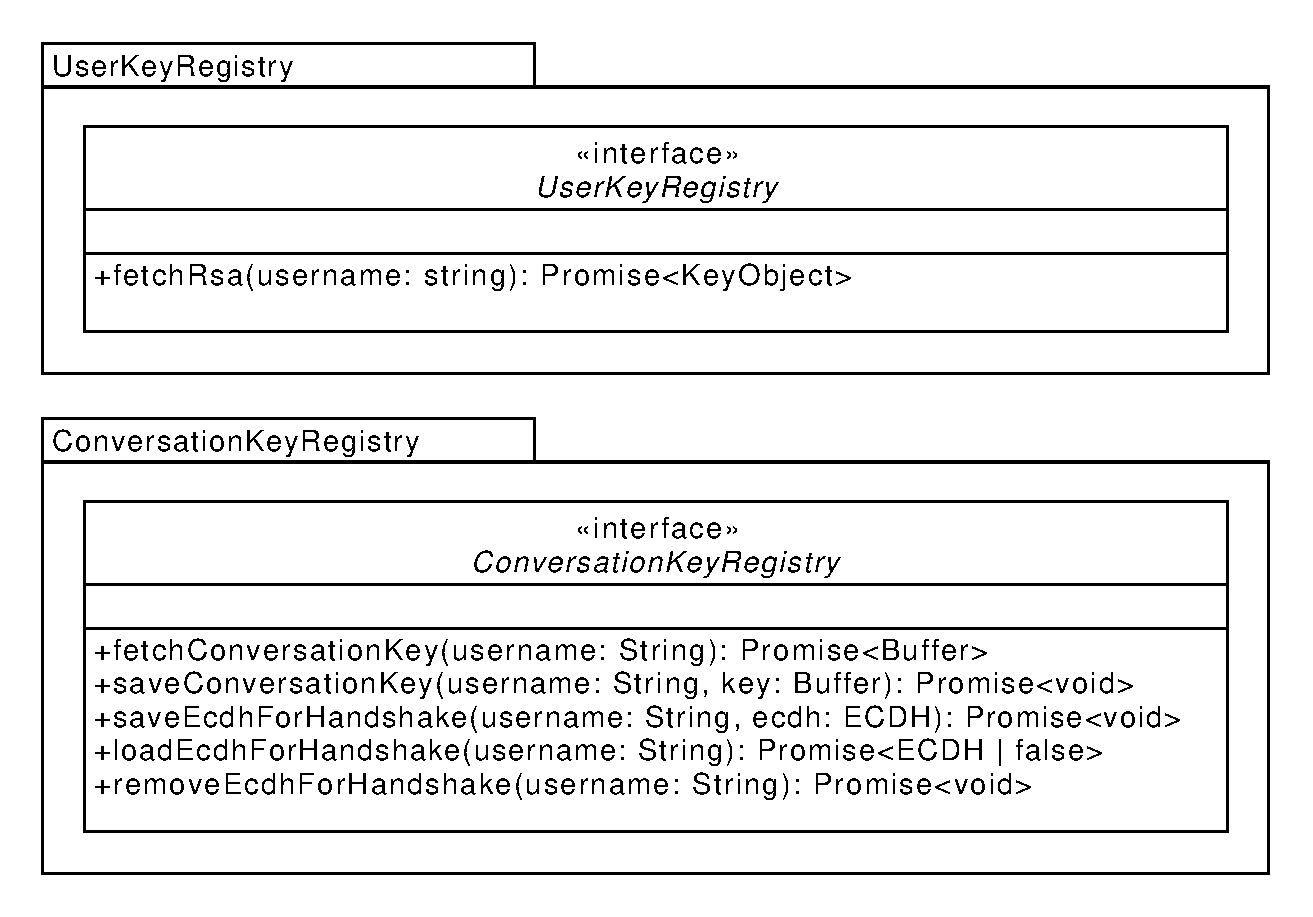
\includegraphics[width=1.0\textwidth]{./graphics/classDiagramTransportLibraryDiverse}
    \vspace*{-0.5cm}
    \caption{Trale key registry interfaces}
    \label{fig:figure34}
\end{figure}

\paragraph{Message abstraction}
The following diagram~\ref{fig:figure35} shows the abstraction layer for Trale messages.
Since we have to work with network connections, which do not support transmitting high-level objects, we instead have
to send binary data.
This package aims to make handling messages in either format easier by providing a simple yet powerful \ac{api} to
easily convert between high-level message objects and raw binary data.
By utilizing enumerations we save a bunch of resources since we only have to send an integer to indicate a message type
but are able to use an expressive name in our code to avoid confusion and provide easy extensibility.
This enables us to later implement further message types (e.g.\ file transfers(e.g.\ .pdf), videos, photos, etc.).

It also, provides the ability for senders to attach their own signature so that the receiver is able to verify that the
message has not been modified during transportation and originates from the proper sender.

\begin{figure}[H]
    \centering
    \caption{Trale message abstraction for low-level operations}
    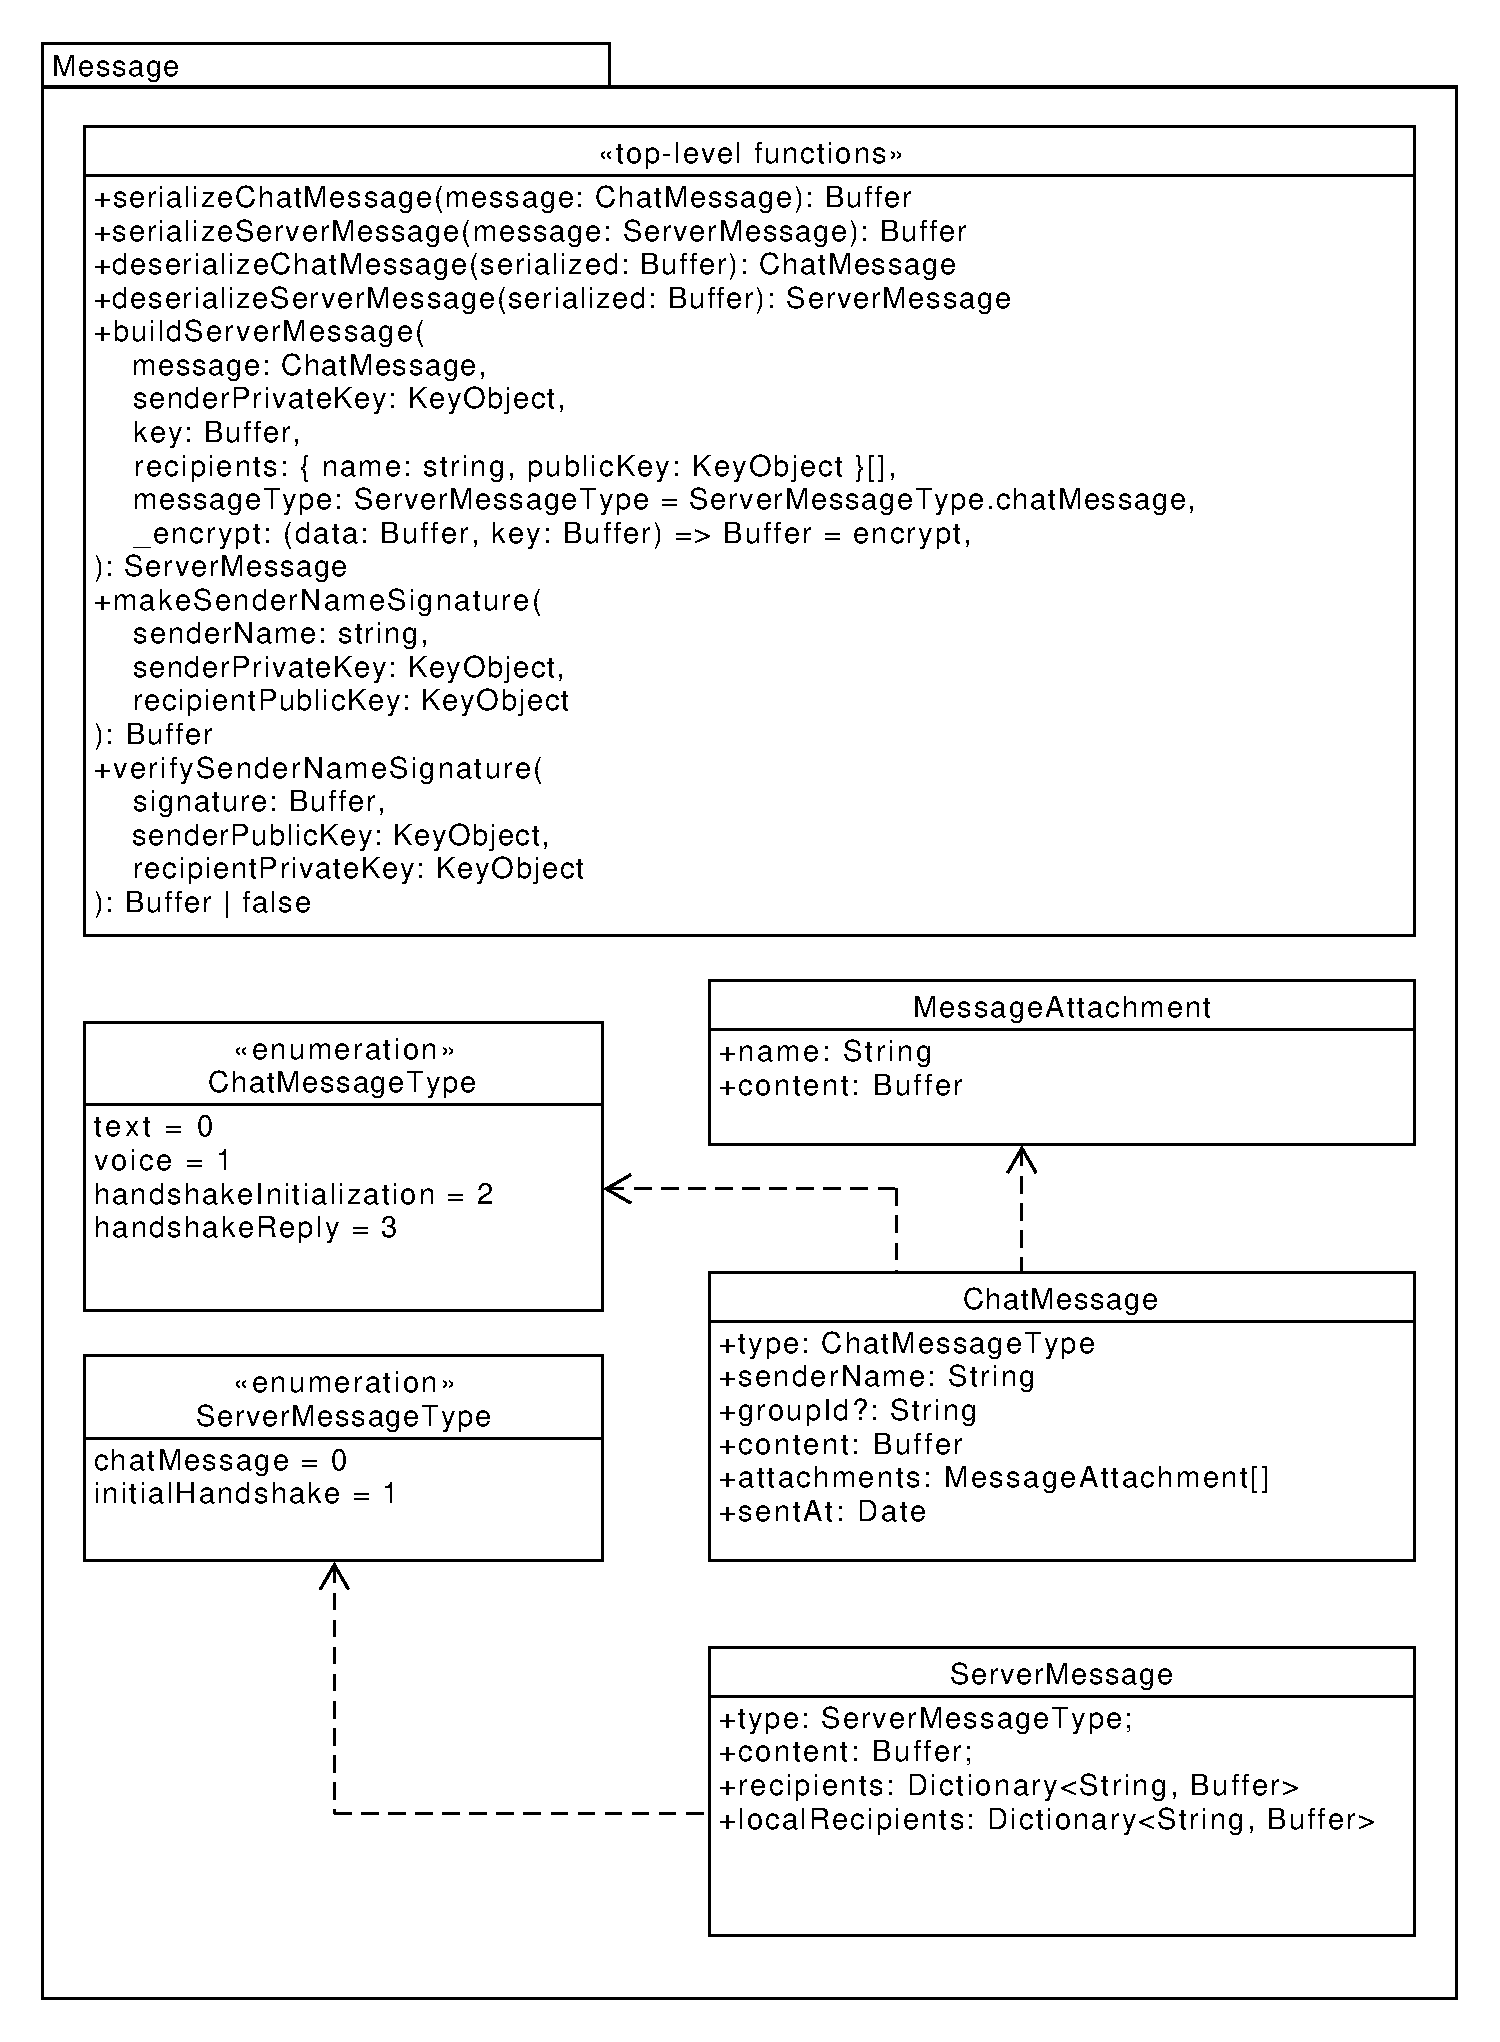
\includegraphics[width=1.0\textwidth]{./graphics/classDiagramTransportLibrary-Message}
    \label{fig:figure35}
\end{figure}

\paragraph{Trale Server}
The following diagram~\ref{fig:figure36} shows the Trale server, and the corresponding client bus.

The Trale server package serves two main purposes.
First, the \ac{titp} server itself, which is responsible for verifying incoming connections and establishing a secure
tunnel with those new connections.

Second, the client bus, which is responsible for distributing messages to users who are online and notifying the library
consumer to persist the messages of users who are offline.

\begin{figure}[H]
    \centering
    \caption{Trale server library package}
    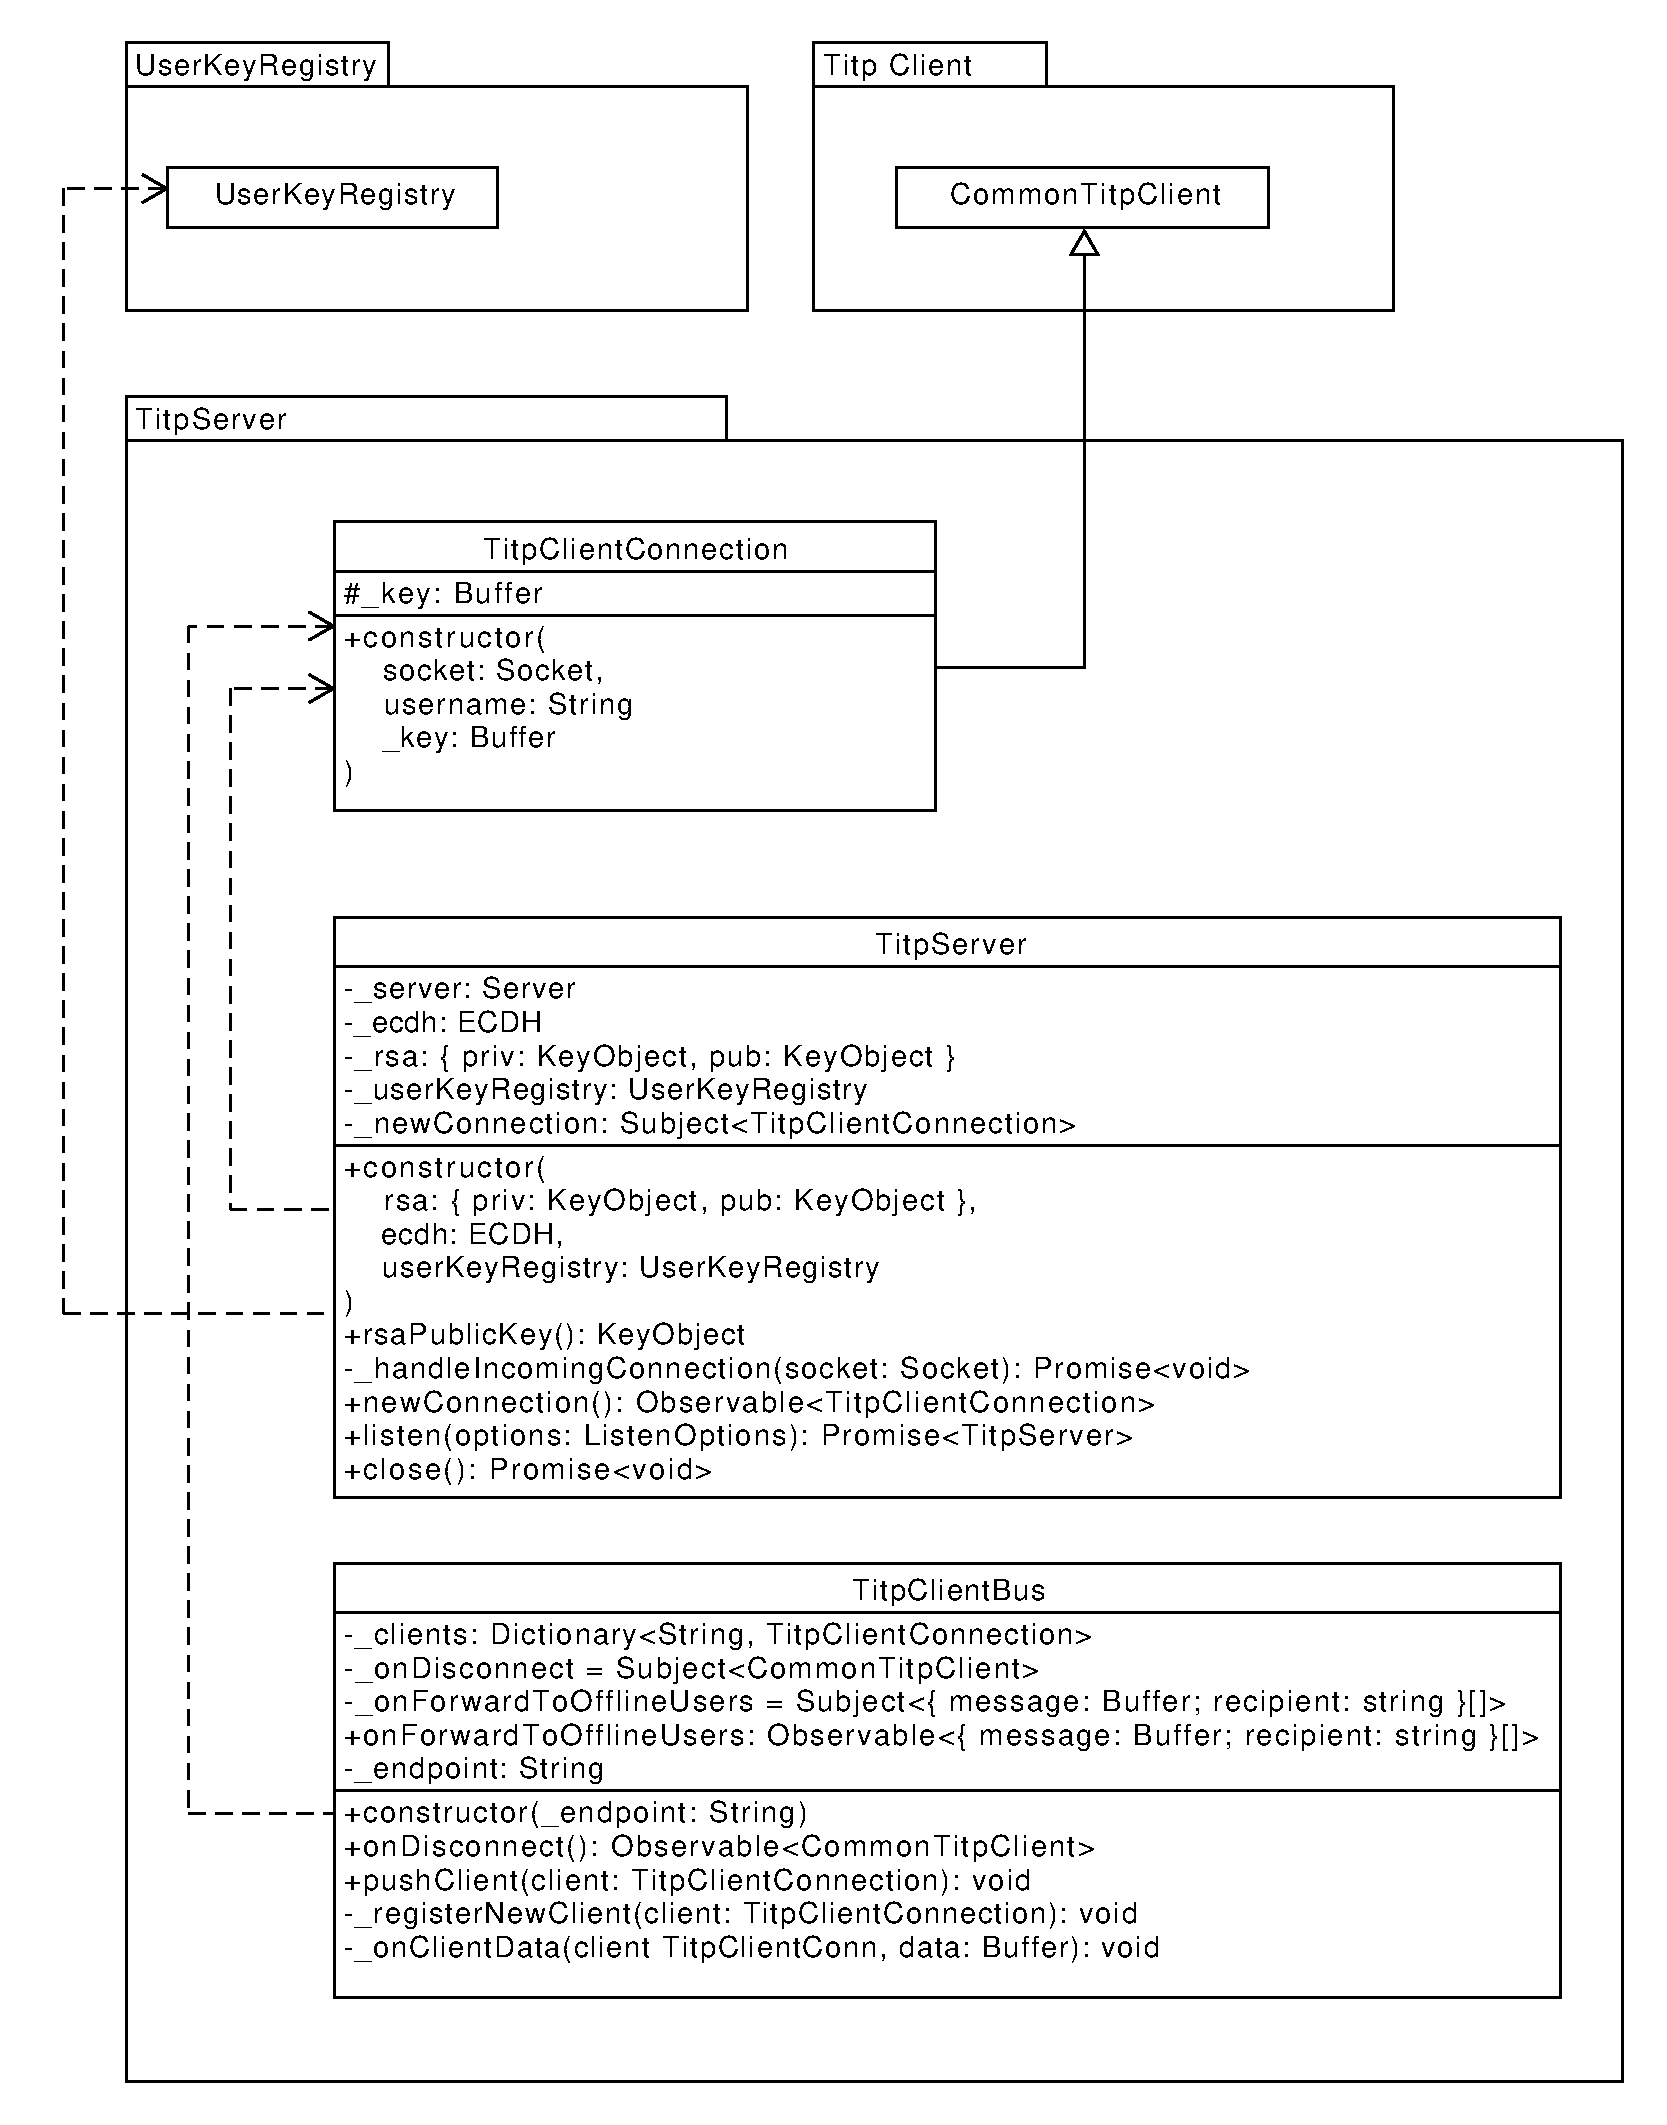
\includegraphics[width=1.0\textwidth]{./graphics/classDiagramTransportLibrary-Server}
    \label{fig:figure36}
\end{figure}

\paragraph{Trale Transport Client}
The foundation of the Trale transport client builds the abstract \textit{CommonTitpClient} class (\ref{fig:figure37}).
It is utilized by the server as well as the client application, as both parts need lots of the same logic.
This logic mainly includes the secure send and receive procedures for data.
The \textit{CommonTitpClient} builds a wrapper around a raw socket connection.
In comparison to regular sockets we are not transferring a continuous stream of data, but rather packages of data.
Those packages of bytes start with the length of the full package to indicate how many of the following bytes belong to
one package.
This is necessary in order to properly decrypt and deserialize the messages that will be transferred via this
connection.

The \textit{TitpClient} implementation will be utilized in the actual application parts.
It provides a higher abstraction level on which directly chat messages can be extracted from a connection instead of
having to manually parse them from the \textit{data()} observable.
Further, the \textit{TitpClient} provides the option to directly send a message to a set of users.
The implementation will take care of serialization on its own.

Further, the \textit{TitpClient} is able to initialize the key negotiation via \ac{ecdh} with another user.
The handshake procedure is designed as a state machine, so it can be easily extended in the future, if further steps will
become necessary.
In case the client receives an incoming handshake, it will automatically calculate a shared secret and reply with its
own \ac{ecdh} public key.

It also provides a \textit{connect()} method which takes care of connecting to the server and performing the handshake
to establish a secure connection.

\begin{figure}[H]
    \centering
    \caption{Trale client library package}
    \hspace*{-2.9cm}
    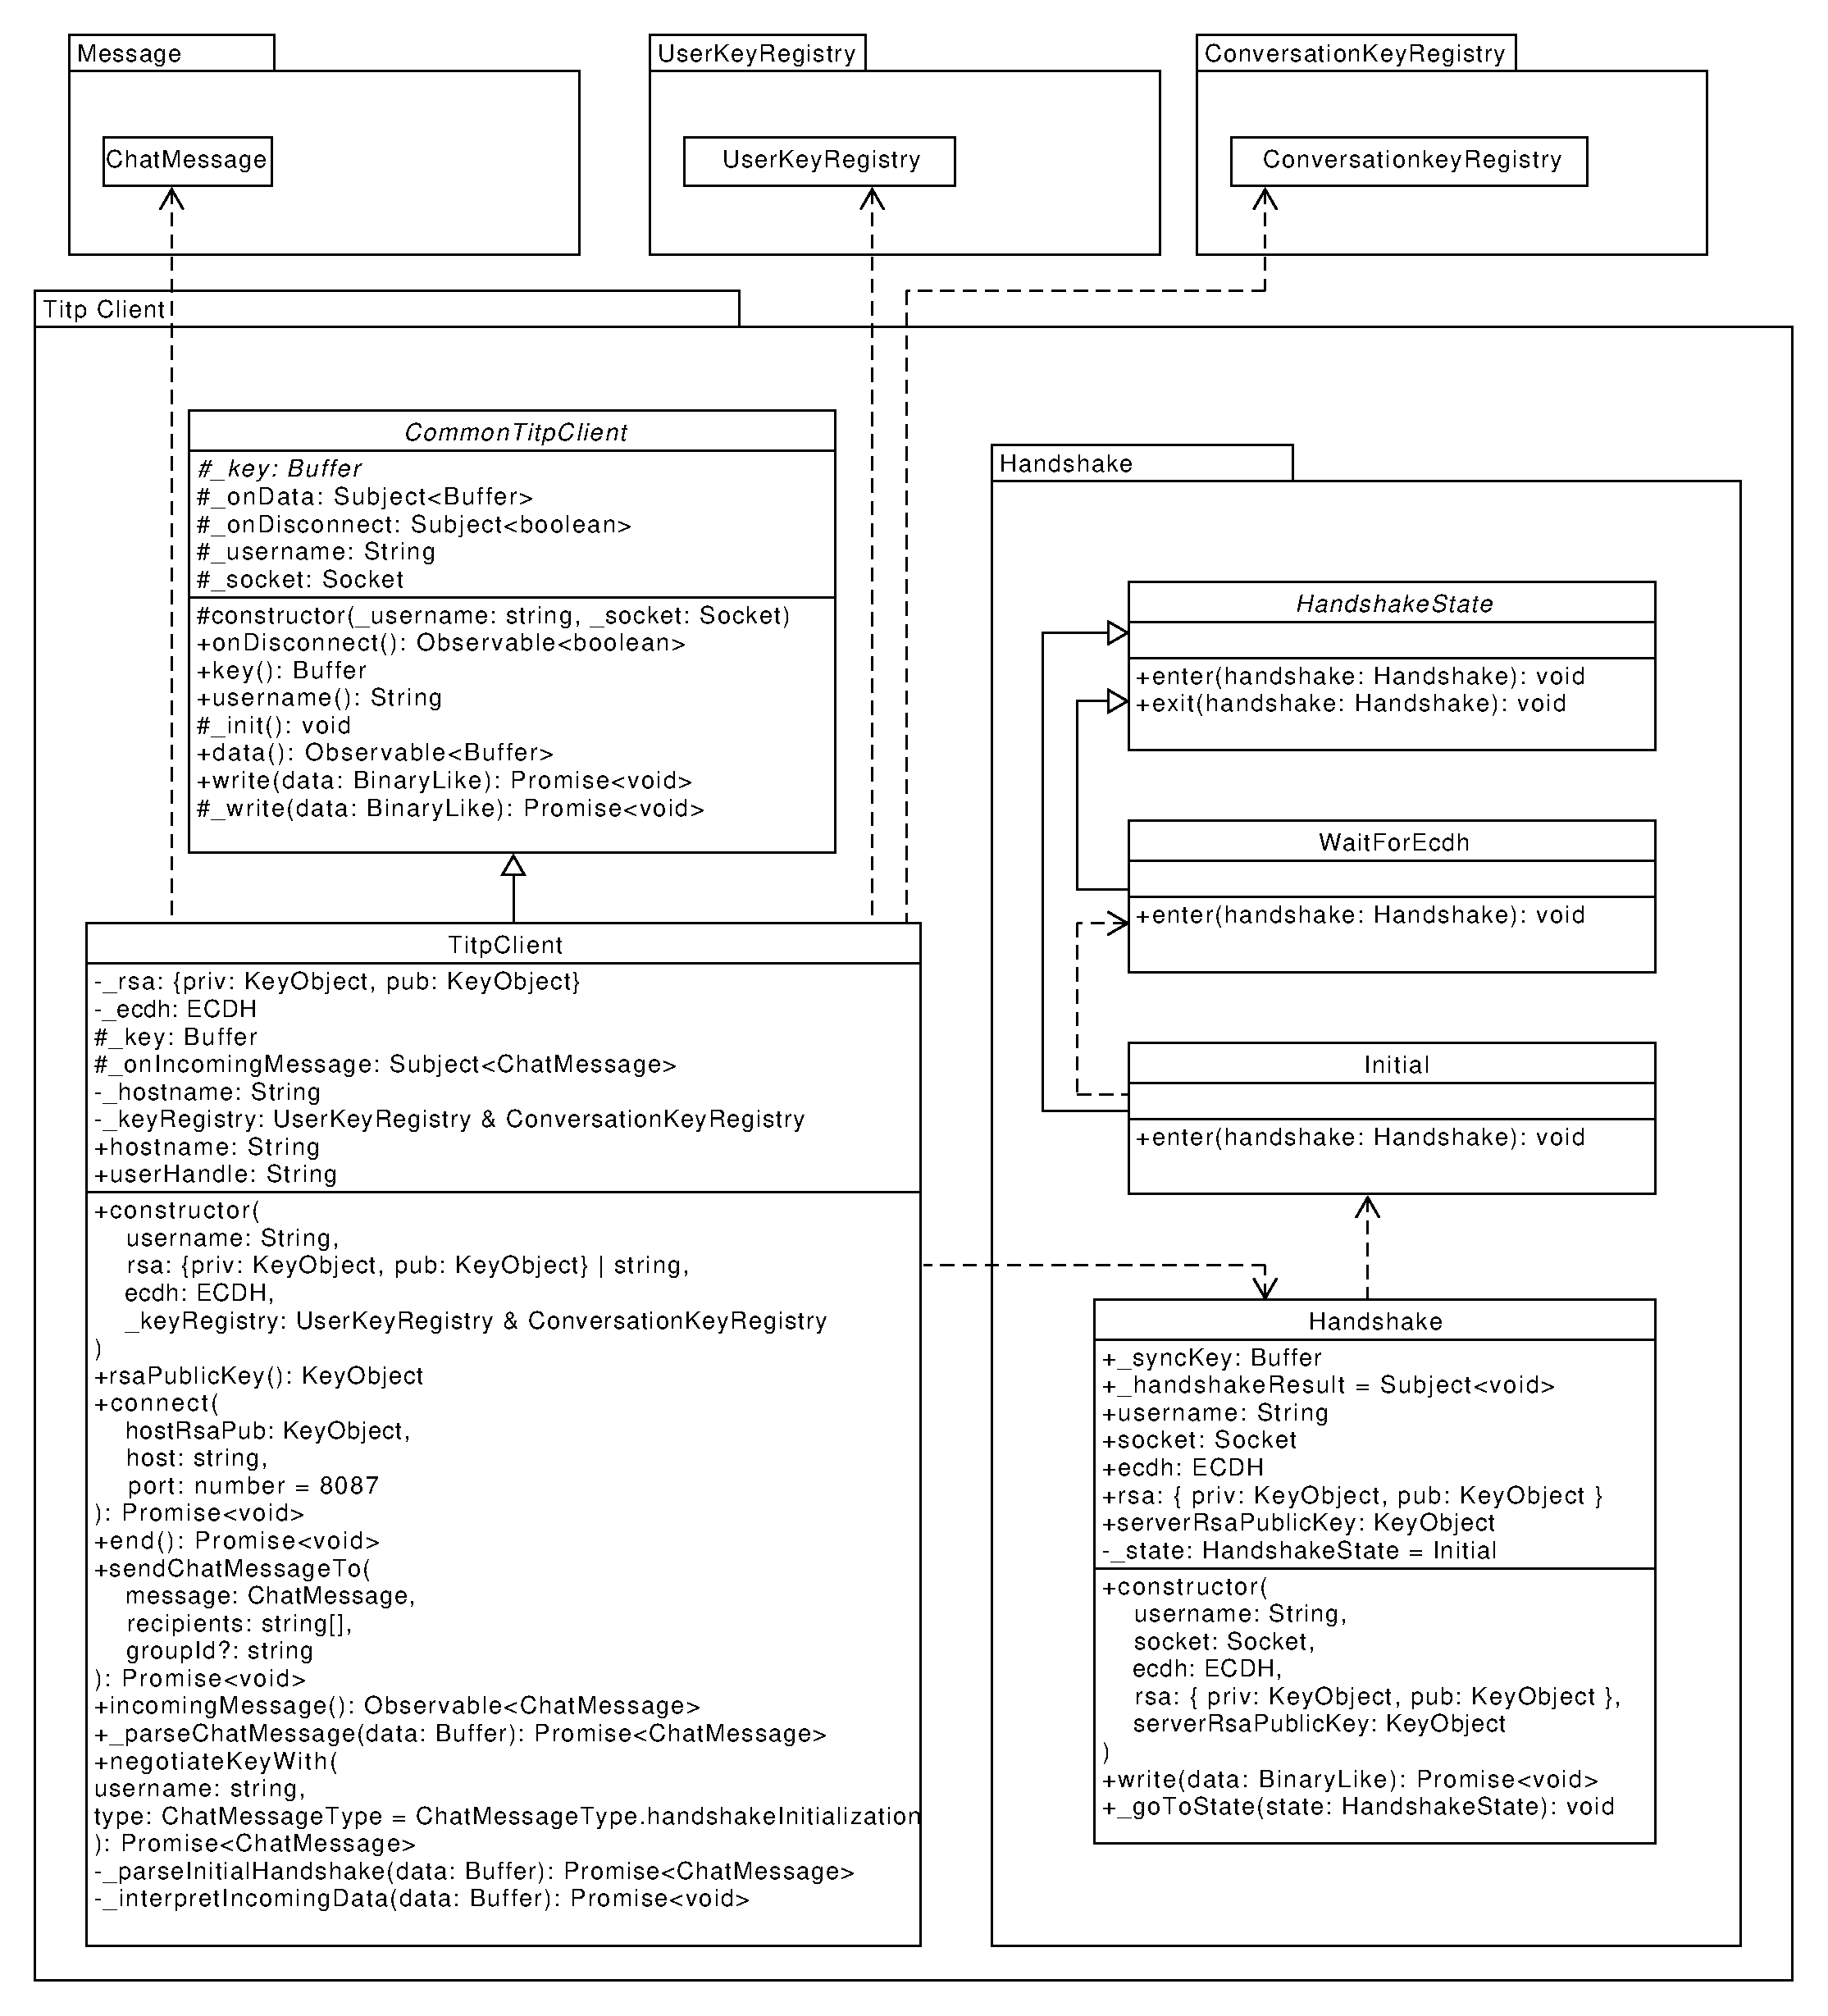
\includegraphics[width=1.3\textwidth]{./graphics/classDiagramTransportLibrary-TitpClient}
    \label{fig:figure37}
\end{figure}

\subsubsection{Persistence Library}

\paragraph{Crypto Storage \ac{api}}

The crypto storage \ac{api} provides a simple and intuitive way to read and write data to a local directory.
A base directory as the root for all operations is set centrally during the initialization of the crypto storage
(~/.trale).
This is very useful in order to abstract away the necessity to know the full path to the file one is trying to access.
Since our application aims to run on as many platforms as possible, it also removes the necessity to remove the path
separator on a given operating system (e.g.\ Windows \enquote{\textbackslash} vs.\ Linux \enquote{/}).

Additionally, the crypto storage manages the encryption and decryption of files automatically, while the desired
mechanism of said encryption and decryption can be set by the one instantiating the crypto storage.

\paragraph{Text Record Storage}

In addition to the crypto storage \ac{api}, the text record storage is able to load files partially line by line.
The lines are accessed as last-in first-out (LIFO).
This is especially useful in our use-case, since we are going to use the text record storage to save and load chat
messages.
The most important reason to do so however, is \ac{ram} efficiency.
We could also load an entire chat via the crypto storage but on a long chat this would be a waste of memory as not all
messages are needed as soon as one opens a chat.
Therefore, the text record storage only loads the latest messages as soon as they are requested.
If nothing is requested, no data will be loaded and no \ac{ram} will be wasted.
\begin{figure}[H]
    \centering
    \caption{Trale persistence library package}
    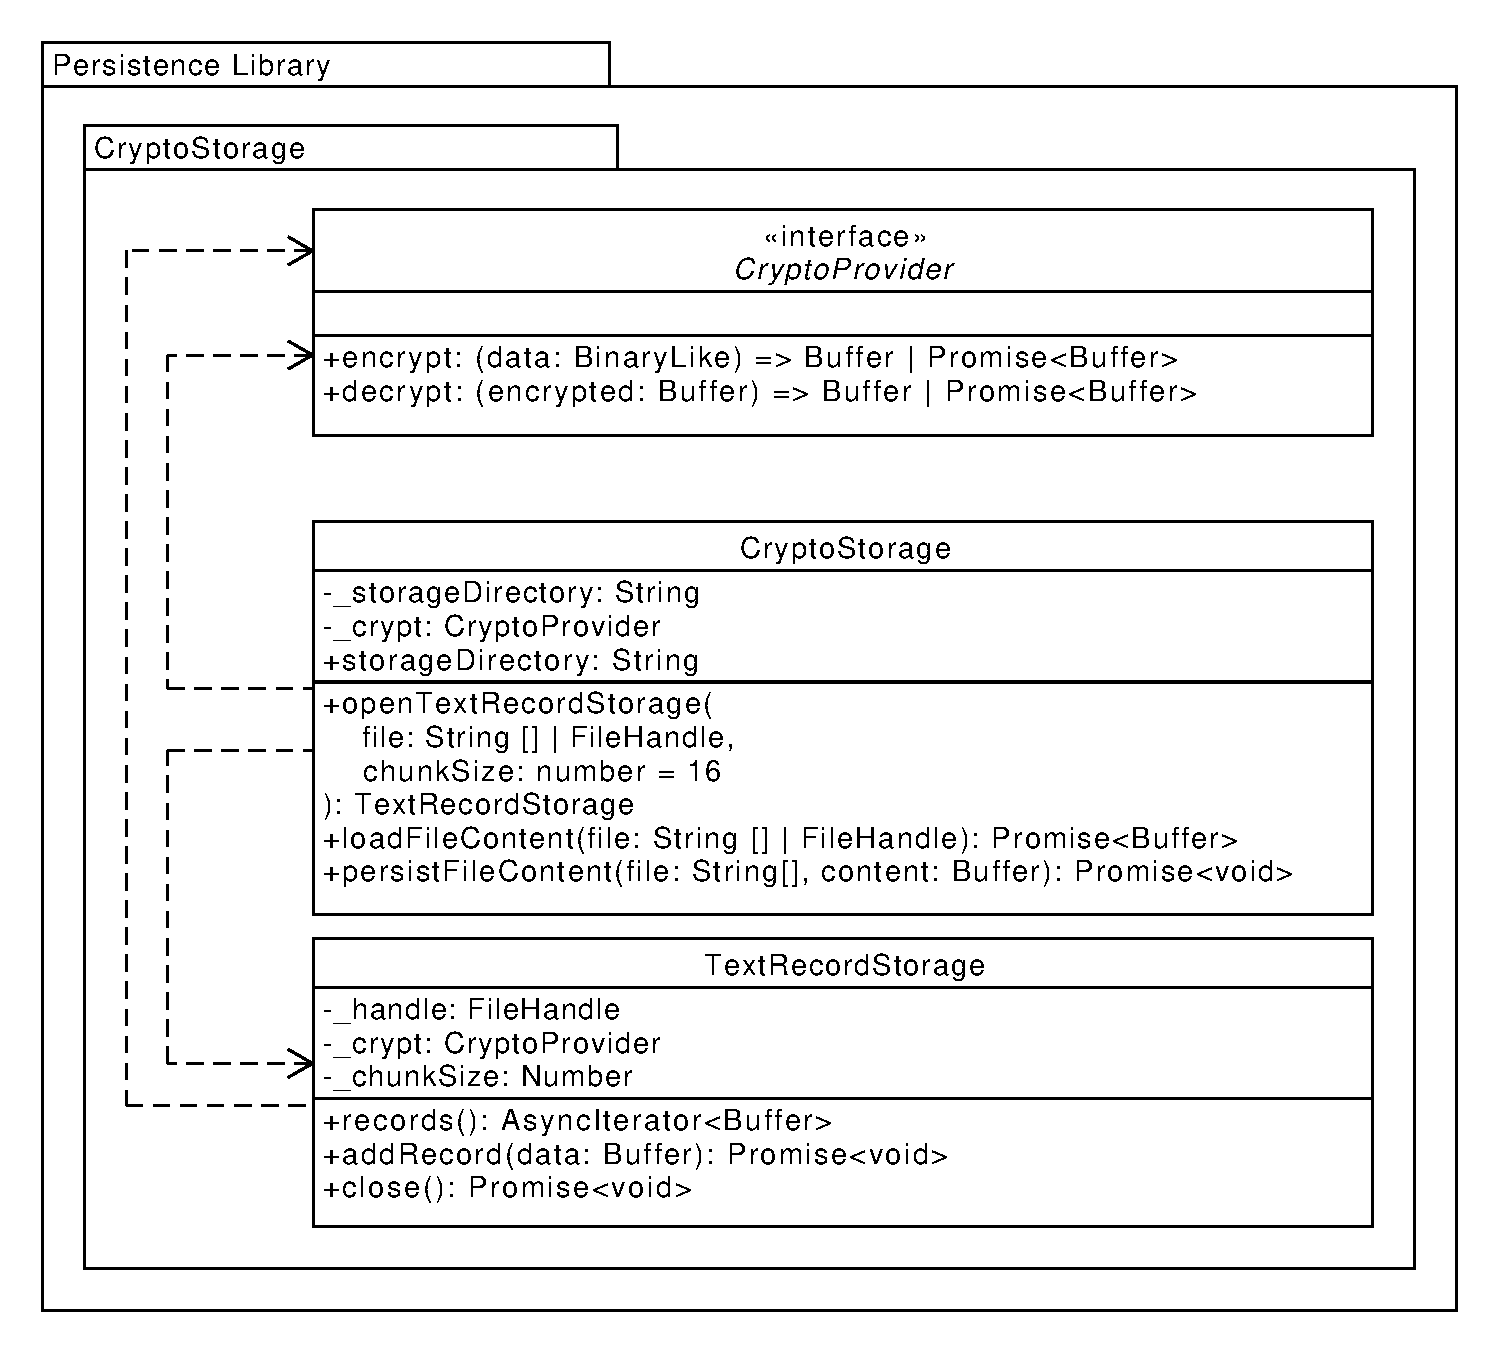
\includegraphics[width=1\textwidth]{./graphics/classDiagramPersistenceLibrary}
    \label{fig:figure38}
\end{figure}

\subsubsection{Utilities Library}
The utilities library contains various functionality which is of general use and not as specific as logic contained in
prior libraries.
It basically serves as a collection of shared code, which is used in all backend services as well as the frontend
client.
This functionality includes common helpers for security, express.js, and common data types.

\begin{figure}[H]
    \centering
    \caption{Trale utilities library package}
    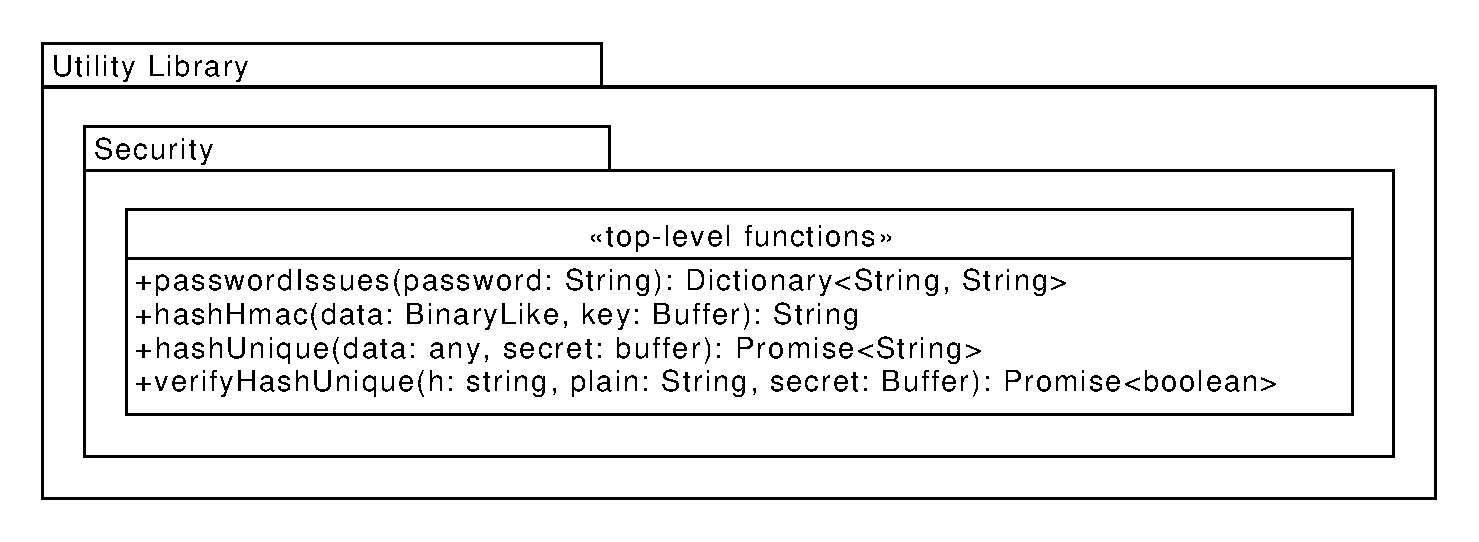
\includegraphics[width=1\textwidth]{./graphics/classDiagramUtilitiesLibrary}
    \label{fig:figure39}
\end{figure}
